\newcommand{\figureIICSchematics}[1]{
  \def\lang{\detokenize{#1}}
  \def\langRu{\detokenize{ru}}
  \def\langEn{\detokenize{en}}
  \def\figureCaption{XXX: No translation.}
  \ifx \lang\langRu
  \def\figureCaption{
    Устройство шины \gls{I2C}.
  }
  \fi
  \if \lang\langEn
  \def\figureCaption{
    \gls{I2C} architecture.
  }
  \fi
  \begin{figure}[H]
    \centering
    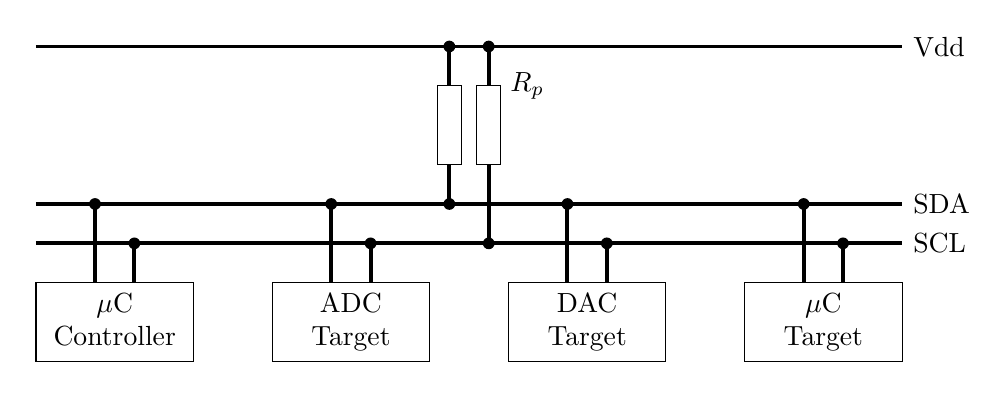
\begin{tikzpicture}
      \draw[draw=black] (0, 2) rectangle ++(2, 1) node[pos=.5] {%
        \begin{tabular}{c}%
          $\mu$C\\Controller%
      \end{tabular}};
      \draw[draw=black] (3, 2) rectangle ++(2, 1) node[pos=.5] {
        \begin{tabular}{c}
          ADC\\Target
      \end{tabular}};
      \draw[draw=black] (6, 2) rectangle ++(2, 1) node[pos=.5] {
        \begin{tabular}{c}
          DAC\\Target
      \end{tabular}};
      \draw[draw=black] (9, 2) rectangle ++(2, 1) node[pos=.5] {
        \begin{tabular}{c}
          $\mu$C\\Target
      \end{tabular}};

      %% Horizontal lines.
      \draw [line width=0.5mm] (0, 3.5) -- (11, 3.5) node[right] {SCL};
      \draw [line width=0.5mm] (0, 4.0) -- (11, 4.0) node[right] {SDA};
      \draw [line width=0.5mm] (0, 6.0) -- (11, 6.0) node[right] {Vdd};

      %% Vertical lines.
      \foreach \a/\b in {0.75/1.25, 3.75/4.25, 6.75/7.25, 9.75/10.25} {
        \draw [line width=0.5mm] (\a, 3) -- (\a, 4) node[circle,fill,inner sep=1.5pt]{};
        \draw [line width=0.5mm] (\b, 3) -- (\b, 3.5) node[circle,fill,inner sep=1.5pt]{};
      };

      \draw[line width=0.5mm] (5.25, 4) node[circle,fill,inner sep=1.5pt]{}
      -- (5.25, 6) node[circle,fill,inner sep=1.5pt]{};
      \draw[line width=0.5mm] (5.75, 3.5) node[circle,fill,inner sep=1.5pt]{}
      -- (5.75, 6) node[circle,fill,inner sep=1.5pt]{};

      \draw[draw=black, fill=white] (5.1, 4.5) rectangle ++(0.3, 1);
      \draw[draw=black, fill=white] (5.6, 4.5) rectangle ++(0.3, 1) node[right] {$R_p$};

    \end{tikzpicture}
    \caption{\figureCaption}
    \label{fig:i2c-schematics}
  \end{figure}
}
